\documentclass[10pt]{beamer}

\usetheme{default}

\usepackage[utf8]{inputenc}
\usepackage[russian]{babel}
\usepackage[OT1]{fontenc}
\usepackage{amsmath}
\usepackage{amsfonts}
\usepackage{amssymb}
\usepackage{graphicx}
\usepackage{etoolbox}
\usepackage{caption}
\usepackage{subcaption}
\usepackage{pifont}
\usepackage{xcolor}
\usepackage{framed}
\definecolor{shadecolor}{cmyk}{0,0,0,1}

\makeatletter

\setbeamercolor{title}{fg=white}
\setbeamercolor{frametitle}{fg=black}
\setbeamerfont*{title}{family=\sffamily,size=\LARGE}

\setbeamerfont{page number in head/foot}{size=\scriptsize}
\setbeamertemplate{footline}[frame number]
\let\otp\titlepage
\renewcommand{\titlepage}{\otp\addtocounter{framenumber}{-1}}

\setbeamertemplate{background canvas}{%
	\ifnumequal{\c@framenumber}{0}{%
      
\includegraphics[width=\paperwidth,height=\paperheight]{images/cover.png}
   }{%
      \ifnumequal{\c@framenumber}{\inserttotalframenumber}{
         
\includegraphics[width=\paperwidth,height=\paperheight]{images/back.png}
      }{%
         % Other frames
      }%
   }%
}

\makeatother

\beamertemplatenavigationsymbolsempty

\author{Николай Анохин}
\title{\newline \newline \newline Лекция 4 \\ Задача классификации}

\begin{document}

\begin{frame}[plain]
\titlepage
\end{frame}

\begin{frame}{План занятия}
\tableofcontents
\end{frame}

% ========================================
\section{Задачи классификации и регрессии}
% ========================================

\begin{frame}{Классификация: интуиция}

\begin{block}{Задача}
Разработать алгоритм, позволяющий определить класс произвольного объекта из некоторго множества
\begin{itemize}
\item Дана {\it обучающая выборка}, в которой для каждого объекта известен класс
\end{itemize}
\end{block} 

\begin{center}
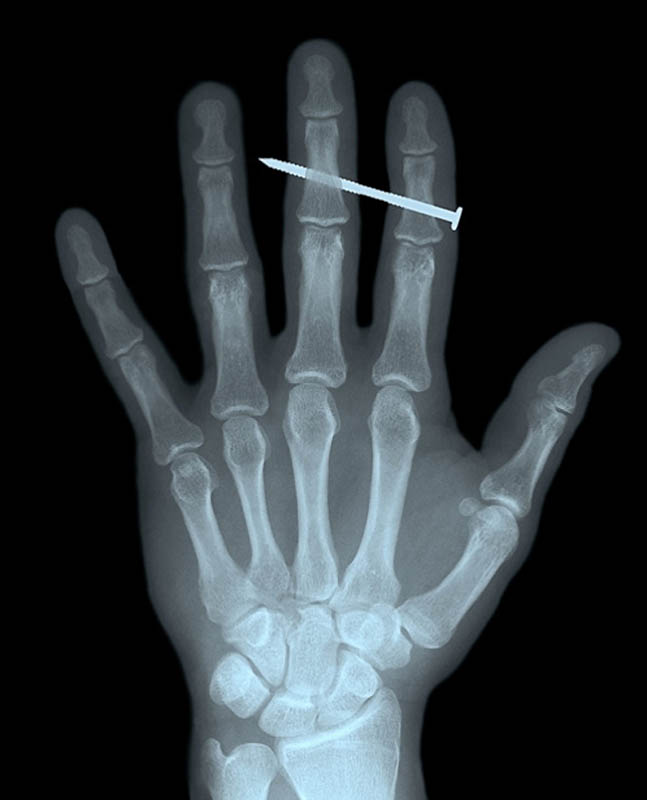
\includegraphics[scale=0.15]{images/xray.jpg}
\end{center}

\end{frame}

% ============================================== %

\begin{frame}{Регрессия: интуиция}

\begin{block}{Задача}
Разработать алгоритм, позволяющий предсказать числовую характеристику произвольного объекта из некоторого множества
\begin{itemize}
\item Дана {\it обучающая выборка}, в которой для каждого объекта известно значение данной числовой характеристики
\end{itemize}
\end{block}

\begin{center}
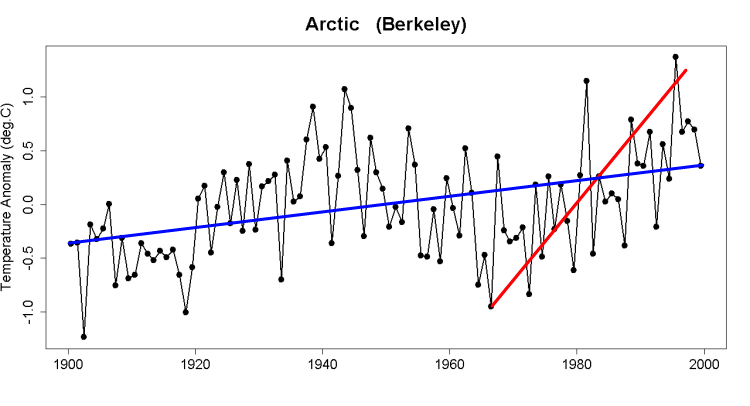
\includegraphics[scale=0.3]{images/kioto.png}
\end{center}

\end{frame}

\begin{frame}{Постановка задачи}

\[
	H = \{h(\mathbf{x}, \theta): \mathcal{X} \times \Theta \rightarrow \mathcal{Y} \}
\]

\end{frame}

% ========================================
\section{Подходы к моделированию}
% ========================================

\begin{frame}{}

\end{frame}

% ========================================
\section{Теория принятия решений}
% ========================================

\begin{frame}{}

\end{frame}

% ========================================
\section{Оценка результатов классификации}
% ========================================

\begin{frame}{}

\end{frame}

% ========================================
\section{Деревья решений}
% ========================================

\begin{frame}{}

\end{frame}

\begin{frame}[plain]
\begin{center}
{\Large Вопросы}
\end{center}
\end{frame}

\end{document}